\chapter*{‌پیوست}
\markboth{پیوست}{}
\addcontentsline{toc}{chapter}{پیوست}
%موضوعات مرتبط با متن گزارش پایان نامه كه در يكی از گروه‌های زير قرار می‌گيرد، در بخش پيوست‌ها آورده شوند:
%\begin{enumerate}
%\item  اثبات های رياضی يا عمليات رياضی طولانی‌.‌
%\item داده و اطلاعات نمونه (های) مورد مطالعه (\lr{Case Study}) چنانچه طولانی باشد‌.‌
%\item نتايج كارهای ديگران چنانچه نياز به تفصيل باشد‌.‌
%\item مجموعه تعاريف متغيرها و پارامترها، چنانچه طولانی بوده و در متن به انجام نرسيده باشد‌.‌
%\end{enumerate}
% براي شماره‌گذاري روابط، جداول و اشكال موجود در پيوست‌ از ساختار متفاوتي نسبت به متن اصلي استفاده مي‌شود كه در زير به‌عنوان نمونه نمايش داده شده‌است. 
% \begin{equation}
%F=ma
%\end{equation}
\section*{الف} \label{apendix:mpu}
\begin{figure}[h!]
	\centering
	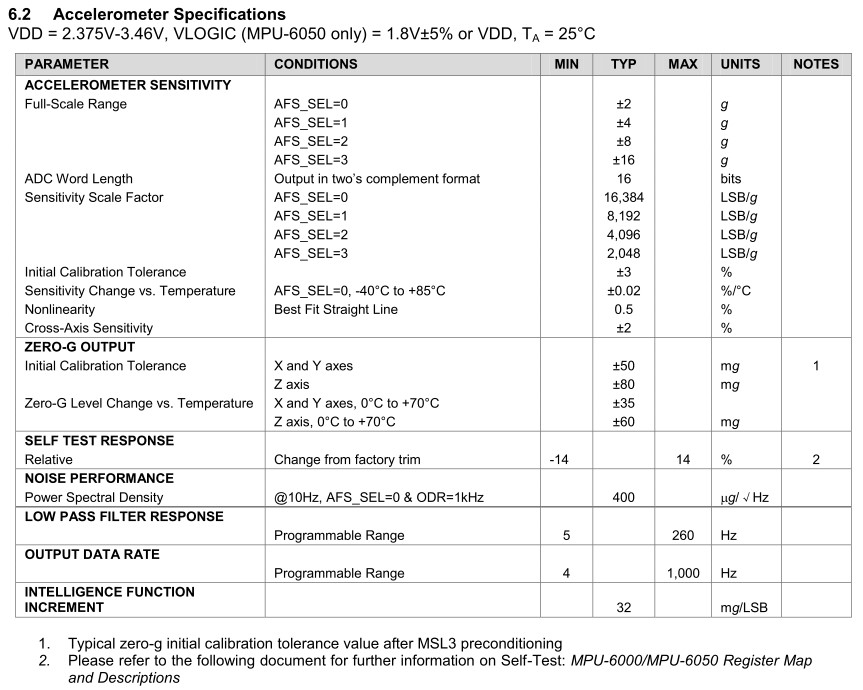
\includegraphics[width=\linewidth]{ds_accel}
	%\caption{تصویر محل اتصال \lr{USB} در بدنه}
	%\label{fig:ds-mpu}
\end{figure}
\begin{figure}[h!]
	\centering
	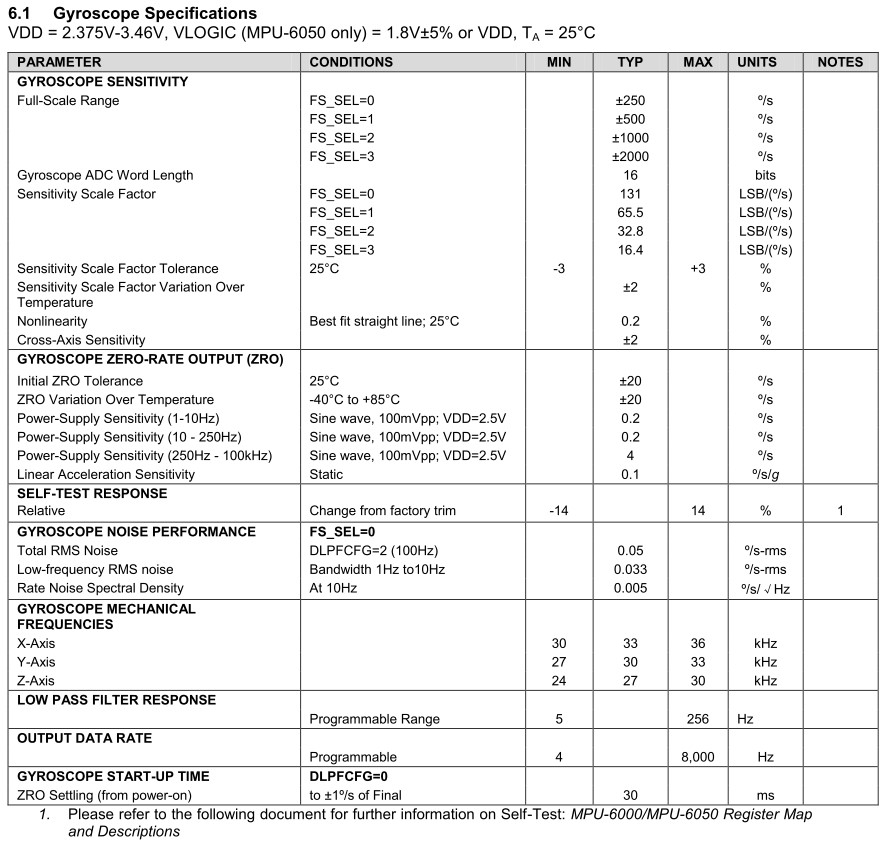
\includegraphics[width=\linewidth]{ds_gyro}
	%\caption{تصویر محل اتصال \lr{USB} در بدنه}
	%\label{fig:ds-mpu}
\end{figure}
\begin{figure}[h!]
	\centering
	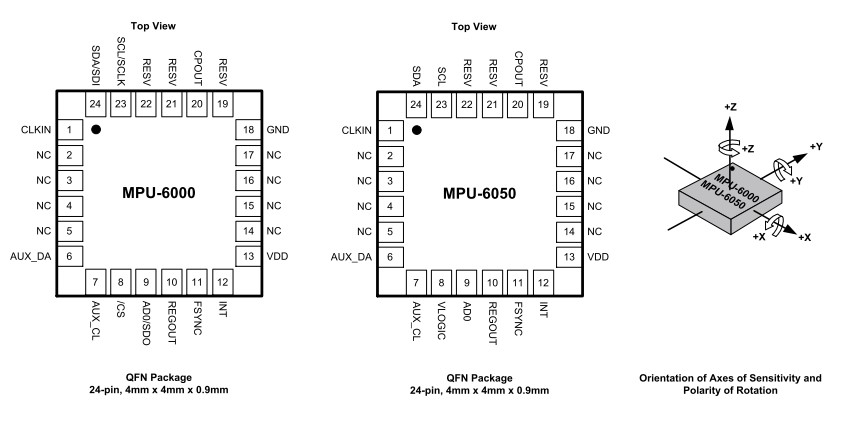
\includegraphics[width=\linewidth]{ds_mpu}
	%\caption{تصویر محل اتصال \lr{USB} در بدنه}
	%\label{fig:ds-mpu}
\end{figure}

\newpage
\section*{ب} \label{apendix:mpu2}
\begin{figure}[h]
	\centering
	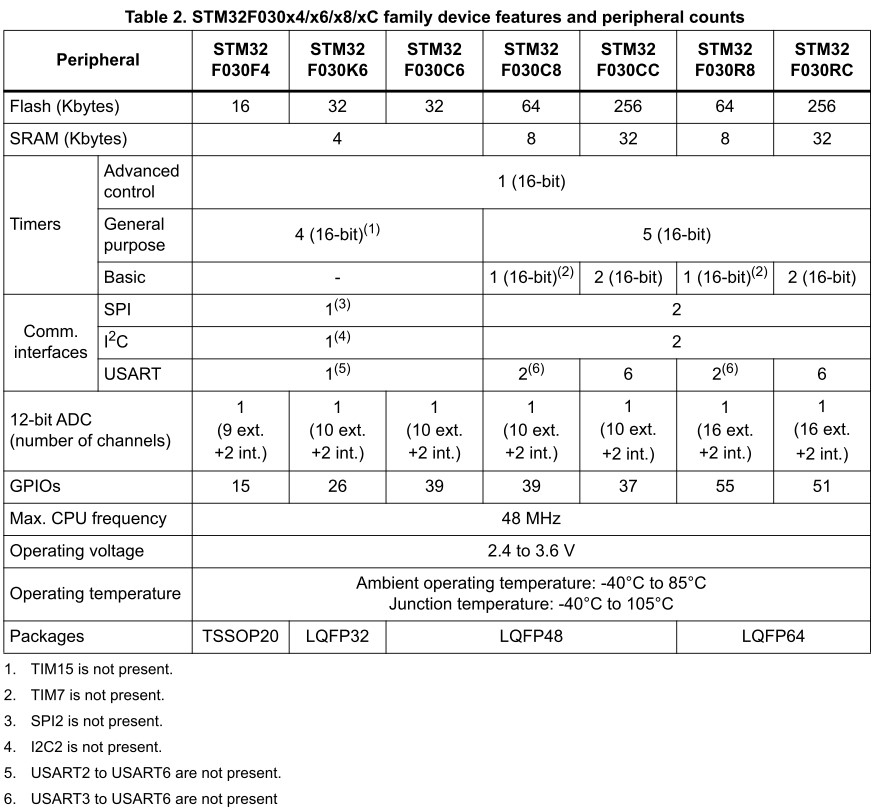
\includegraphics[width=\linewidth]{ds_stm32}
	%\caption{تصویر محل اتصال \lr{USB} در بدنه}
	%\label{fig:ds-mpu}
\end{figure}
